% !TEX root = ../main.tex
\section{The History of Graphical Passwords} \label{sec:historygraphicalpasswords}
	 
  This section will look at related work on graphical passwords from a historical point of view. The graphical password schemes reviewed will provide an elaboration of how the scheme works as well as a graphical illustration of its design

  Since it all started around 1996, there have been many suggestions for graphical password schemes. When proposing a new password scheme, there are several aspects of the scheme that needs to be considered. A password scheme needs to be secure in terms of entropy, and it needs to be hard to guess, as well as being intuitive to use. The history of graphical passwords is important to know because each scheme is attempts to improve various aspects of an earlier proposed scheme. A detailed understanding of today's situation can be understood by studying graphical passwords from a historical point of view. The review starts by looking at where the first graphical passwords originated from, ending up looking at today's situation some of the newly proposed schemes.

  Greg Blonder initially described the idea of graphical passwords in a patent published in 1996 \cite{Blonder}. The graphical password scheme proposed was requiring the user to touch on a predefined set of points on an image to pass the authentication process. The patent was just a proposal and did not further explore the power of graphical passwords, nor did it analyze the security aspects of the patent. Figure \ref{fig:blonder} is an illustration from Blonder's patent of the first graphical password scheme.

    \begin{figure}[H]
      \centering
      \subfigure[Proposal for a graphical password scheme\cite{Blonder}]{
        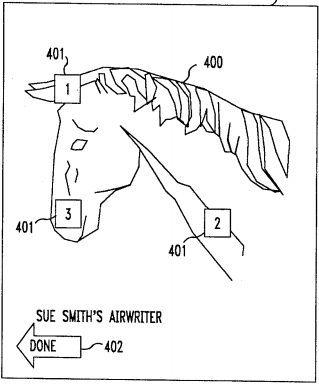
\includegraphics[width=0.30\textwidth]{pics/review/blonder.png}
        \label{fig:blonder}
      }
      \subfigure[DAS \cite{Jermyn}]{
        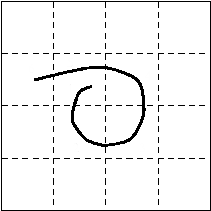
\includegraphics[width=0.30\textwidth]{pics/review/DAS.png}
      \label{fig:DAS}
      }
      \subfigure[BDAS \cite{BDAS}]{
        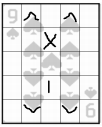
\includegraphics[width=0.30\textwidth]{pics/review/BDAS1.png}
        \label{fig:BDAS}
      }
    \end{figure}

  In 1999, Jermyn et al. \cite{Jermyn} suggested a new graphical password scheme called {\it Draw-a-Secret} (abbreviated DAS). DAS was the first recall-based graphical password scheme proposed. The motivation for the DAS was that graphical input devices enabling the user to decouple the position of inputs from the temporal order in which they occur. The decoupling can be used to generate passwords that increased the size of the password space in practice. In order to make a more memorable password, the research group argued that the DAS was more secure than text-based passwords because the users were able to remember longer and more complex passwords. After the DAS scheme was published, Dunphy and Yan \cite{BDAS} added an extra background image to the DAS and named it "Background DAS" (BDAS). The thought of adding a background to the DAS was to encourage their users to make more complex passwords. Dunphy and Yan believed that the additional image would support the users to remember longer and more complex passwords, and therefore stating that the BDAS was more secure than DAS. Figure \ref{fig:DAS} and Figure \ref{fig:BDAS} are showing images of the DAS and the BDAS respectively.

  In 2000, Dhamija and Perrig \cite{DejaVu} created a new password scheme called {\it Deja Vu}. Deja Vu creates its visual content from the hash visualization technique \cite{HashVisualization}, a technique that replaces meaningless strings with structured images. The images end up looking like random art as a result of the hash visualization technique that turns the bits of a meaningless string into an image. Dhamija and Perrig wanted to make a graphical password scheme that solved some of the shortcomings with recall-based authentication like PINs and text-based passwords. A recall-based authentication scheme is a scheme with the characteristics of {\it something you know}. Dhamija and Perrig designed Deja Vu for purely relying on recognition rather than recall, as well as being hard to write down and share with other people. The images used in Deja Vu makes it hard to share a password because the images are hard to recreate, as well as being easy to remember. Instead of writing art on a grid, the users were asked to select a sequence of images from a random set of images that are generated by the hash visualization technique. The property of being hard to recreate, as well as being easy remember, assists the users in avoiding the habit of writing down the passwords. Figure \ref{fig:DejaVu} are showing the Deja Vu scheme using the hash visualization technique for creating images from random strings looking like random art.

    \begin{figure}[H]
      \centering
      \subfigure[Passfaces \cite{passface}]{
        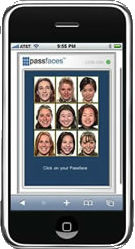
\includegraphics[scale=0.7]{pics/review/Passfaces.jpg}
        \label{fig:Passfaces}
      }
      \subfigure[DejaVu \cite{DejaVu}]{
        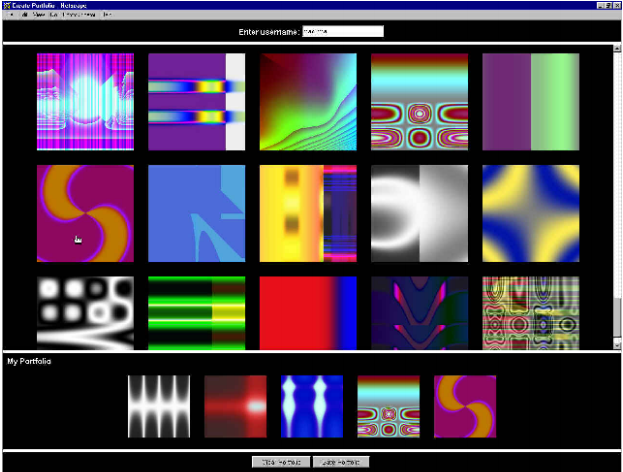
\includegraphics[scale=0.37]{pics/review/DejaVu1.png}
        \label{fig:DejaVu}
      }
    \end{figure}  

  {\it Passfaces} is a graphical password scheme developed by Real User Corporation founded in 2000 \cite{passface}. The Passfaces scheme asks the user first to select four images that are a visualization of human faces. The four faces selected represent the password, and the user is authenticated by identifying them. The selected faces are shown together with eight other faces not initially included in the set of the preselected faces. The scheme exploits the advantage that people are good at recognizing other people, so when users select the human faces they can use the characteristics of the faces in the process of remembering their password. Passfaces are quite similar to the previously described  Deja Vu scheme. The most significant difference between the schemes is that they make use of different association elements in the images, faces, and random art. Figure \ref{fig:Passfaces} illustrates the PassFaces scheme used on a smartphone. Passfaces is one of the few graphical password schemes with a commercial success. 

  Passdoodle was a new scheme first purposed by Goldberg et al. in 2002 and later studied by Varenhorst in 2004 \cite{PassDoodle,Varenhorst}. Passdoodle is similar to DAS, but allows users to create a freehand drawing as a password, and uses a more complex matching process without the visible grid. To add variability to the doodles, additional characteristics like color, drawing speed, and number of pen strokes, have been suggested. Figure \ref{fig:doodle} is an example of a freehand drawn doodle.

  In 2004, Davis et al. did a comparison of a light version of PassFace and a new graphical password scheme called {\it Story} \cite{Davis}. The Story scheme is making the users choosing images to make up a story instead of just recalling a set of faces. The Story scheme was created to help users remember their passwords by making a memorable story of images. For users to pass the authentication process, the story had to be recalled in the correct order. For supporting memorability, users were instructed to construct a story mentally to connect the everyday images in the set. Figure \ref{fig:story} is an image of Story scheme demonstrating the images of objects used to create a story.

  In 2005 Wiedenbeck et al. proposed a graphical password scheme called {\it PassPoints} \cite{Wiedenbeck2}. PassPoints is an extension of Blonder's \cite{Blonder} scheme by eliminating the constraints and allowing arbitrary images to be used. They evaluated their password scheme by testing the scheme for human users. The results showed that PassPoint was a promising scheme with respect to memorability because of the low error rate and low clicking rate. The aim of this study was to gain an understanding of how different images affected user performance in authentication with a graphical password scheme. The preliminary result showed suggested that images may support memorability in graphical password schemes. Figure~\ref{fig:passpoints} is an image of the PassPoints scheme.

    \begin{figure}[H]
      \centering
      \subfigure[Story \cite{Davis}]{
        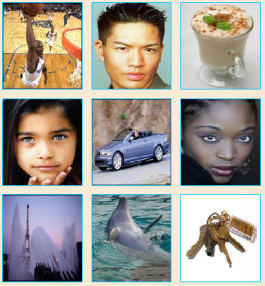
\includegraphics[scale=0.4]{pics/review/story.png}
        \label{fig:story}
      }
      \subfigure[PassPoints \cite{Wiedenbeck2}]{
        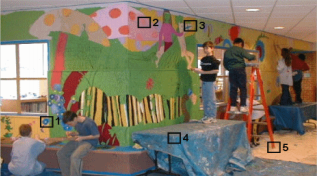
\includegraphics[scale=0.65]{pics/review/passpoint.png}
        \label{fig:passpoints}
      }  
    \end{figure}

  In 2006, a research group wanted to address the problem with graphical passwords and the shoulder surfing problem. They called their password scheme {\it Convex Hull Click} (abbreviated CHC) \cite{Wiedenbeck}. CHC allows the user to use the scheme in secure and insecure locations because users do not directly click on the images in the password. This design makes it hard for attackers to perform a shoulder surfing attack. CHC has a display of small icons. In the authentication process, the user must recognize some minimum number of their chosen images, or {\it pass-icons}, out of a vast number of randomly placed icons. If the user responds correctly every time in the correct order, the user will pass the authentication. Figure~\ref{fig:chc} is a picture of the CHC scheme with three selected icons.

    \begin{figure}[H]
      \centering
      \subfigure[Hand-written Passdoodle \cite{Varenhorst}]{
        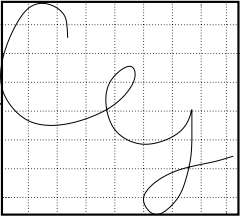
\includegraphics[scale=0.55]{pics/review/doodle.png}
        \label{fig:doodle}
      }
      \subfigure[CHC \cite{Wiedenbeck}]{
        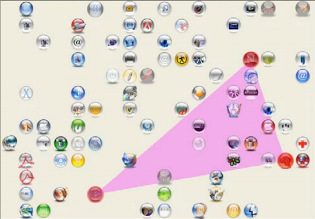
\includegraphics[scale=0.55]{pics/review/CHC.png}
        \label{fig:chc}
      }
    \end{figure}
    
  In 2007, Tao and Adams \cite{Tao} designed the graphical password scheme{\it Pass-Go}. The motivation for creating the Pass-Go scheme was to avoid the problem of failing to be able to accurately recreate the drawing as observed in DAS. Pass-Go reduced the problem by using grid intersection points instead of grid cells as used in DAS. The users movements are captured into grid-lines and intersections, eliminating the possibility to reproduce a password where the difference is too high because of the need for precision in DAS. Figure~\ref{fig:passgo} is an image of the Pass-Go grid used.

  Out of the schemes mentioned until now, most are neither widely known nor widely used. The first known graphical password scheme that has gained increased attention is the Android Unlock pattern. The Android Unlock pattern is a mini version of the ``Pass-Go'' deployed on Google Android smartphones. Rather than entering a four-digit PIN or a text-based password, the user enters a touch-drawn password on a $3\times3$ grid connecting dots forming a password. Figure~\ref{fig:android} is a visualization of the Android Unlock Pattern in use on a smartphone.

    \begin{figure}[H]
      \centering
      \subfigure[Pass-go \cite{Tao}]{
        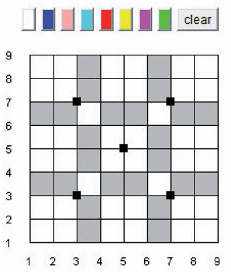
\includegraphics[scale=0.7]{pics/review/passgo2.png}
        \label{fig:passgo}
      }
      \subfigure[Android Unlock Pattern]{
        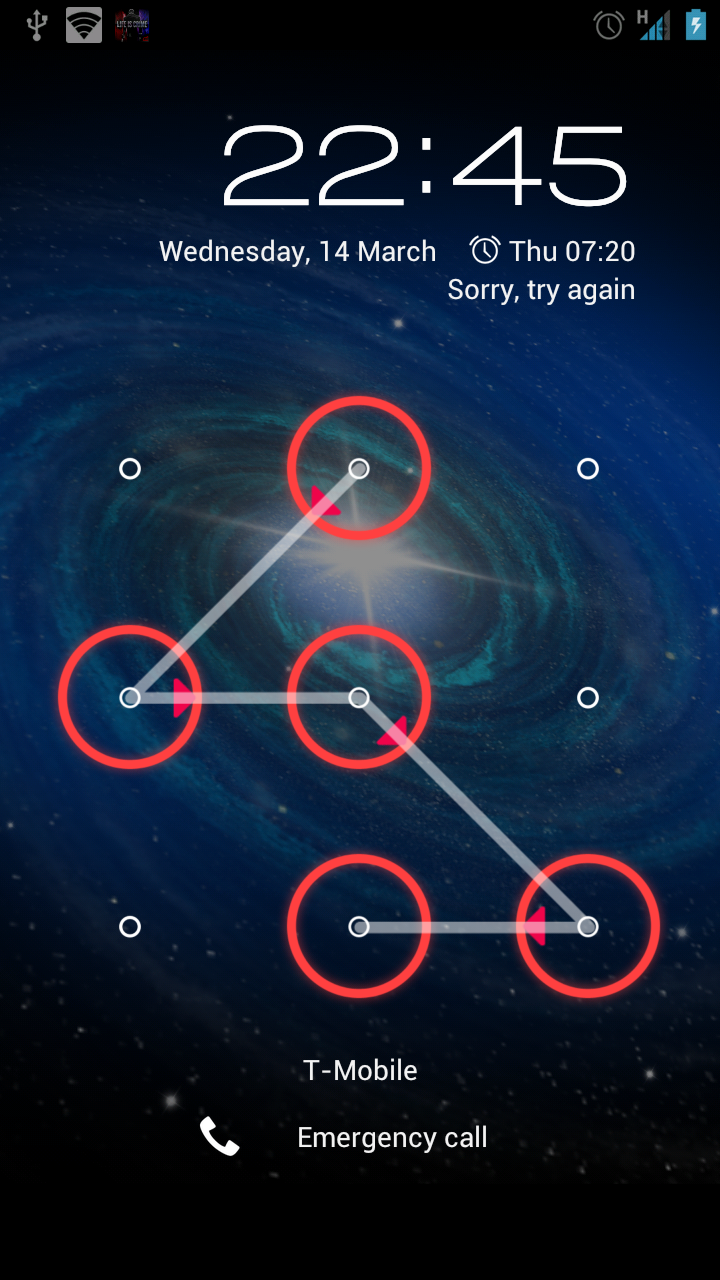
\includegraphics[scale=0.145]{pics/review/patternLock.png}
        \label{fig:android}
      }
    \end{figure}

  Looking at the recently published graphical password we find schemes like GeoPass \cite{GeoPass} and PicassoPass \cite{PicassoPass}. GeoPass uses a digital map for the authentication phase where the user chooses a particular location as their password. PicassoPass is a graphical password scheme presenting a password using a dynamic layered combination of graphical elements. The users can make a story that assists the user in the recognition of the graphical elements. Figure~\ref{fig:geopass} and Figure~\ref{fig:PicassoPass} is the two new proposals for graphical authentication schemes, the GeoPass and the PicassoPass, respectively. 

    \begin{figure}[H]
      \centering
      \subfigure[GeoPass \cite{GeoPass}]{
        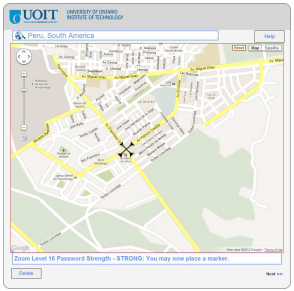
\includegraphics[scale=0.60]{pics/review/geopass.png}
        \label{fig:geopass}
      }
      \subfigure[PicassoPass \cite{PicassoPass}]{
        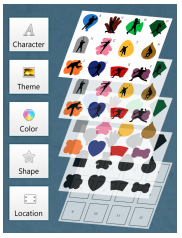
\includegraphics[scale=0.74]{pics/review/picassopass.png}
        \label{fig:PicassoPass}
      }
      \caption{Graphical password schemes}
    \end{figure}
  